\documentclass[../AnalysisNoteJBuxton.tex]{subfiles}
\begin{document}

\subsubsection{Results: \texorpdfstring{$\Lambda$K$^{0}_{S}$ and $\Lambda$K$^{\pm}$: 3 Residual Correlations Included in Fit}{TEXT}}
\label{ResultsLamK_3Res}


\begin{figure}[h]
  \centering
  \includegraphics[width=\textwidth]{\ResultsDirLamKs canKStarCfwFitsLamK0wConj_0010_1030_3050_MomResCrctn_NonFlatBgdCrctn_SingleLamParam_3Res_PrimMaxDecay4fm_UsingXiDataAndCoulombOnly.pdf}
  \caption[\LamALamKs Fits with 3 Residuals]{Fits, with 3 residual correlations included, to the \LamKs (left) and \ALamKs (right) data for the centralities 0-10\% (top), 10-30\% (middle), and 30-50\% (bottom).
The lines represent the statistical errors, while the boxes represent the systematic errors.
Each has unique $\lambda$ and normalization parameters.
The radii are shared amongst like centralities; the scattering parameters ($\mathbb{R}f_{0}$, $\mathbb{I}f_{0}$, $d_{0}$) are shared amongst all.
The black solid line represents the ``raw" fit, i.e. not corrected for momentum resolution effects nor non-flat background.  
The green line shows the fit to the non-flat background.
The purple points show the fit after momentum resolution and non-flat background corrections have been applied.
The initial values of the parameters is listed, as well as the final fit values with uncertainties.
Here, $R$ was restricted to [2.,10.] and $\lambda$ was restricted to [0.1,0.8].}
  \label{fig:LamK0wConjFits_3Res}
\end{figure}

\begin{comment}
\begin{figure}[h]
  \centering
  \includegraphics[width=\textwidth]{\ResultsDirLamKs canKStarCfwFitsLamK0wConj_0010_1030_3050UnZoomed_MomResCrctn_NonFlatBgdCrctn_SingleLamParam_3Res_PrimMaxDecay4fm_UsingXiDataAndCoulombOnly.pdf}
  \caption[\LamALamKs Fits with 3 Residuals (Wide Range)]{Same as Fig. \ref{fig:LamK0wConjFits_3Res}, but with a wider range of view.  
Fits, with 3 residual correlations included, to the \LamKs (left) and \ALamKs (right) data for the centralities 0-10\% (top), 10-30\% (middle), and 30-50\% (bottom).
The lines represent the statistical errors, while the boxes represent the systematic errors.
Each has unique $\lambda$ and normalization parameters.
The radii are shared amongst like centralities; the scattering parameters ($\mathbb{R}f_{0}$, $\mathbb{I}f_{0}$, $d_{0}$) are shared amongst all.
The black solid line represents the ``raw" fit, i.e. not corrected for momentum resolution effects nor non-flat background.  
The green line shows the fit to the non-flat background.
The purple points show the fit after momentum resolution and non-flat background corrections have been applied.
The initial values of the parameters is listed, as well as the final fit values with uncertainties.
Here, $R$ was restricted to [2.,10.] and $\lambda$ was restricted to [0.1,0.8].}
  \label{fig:LamK0wConjFitsUnZoomed_3Res}
\end{figure}
\end{comment}

\begin{figure}[h]
  \centering
  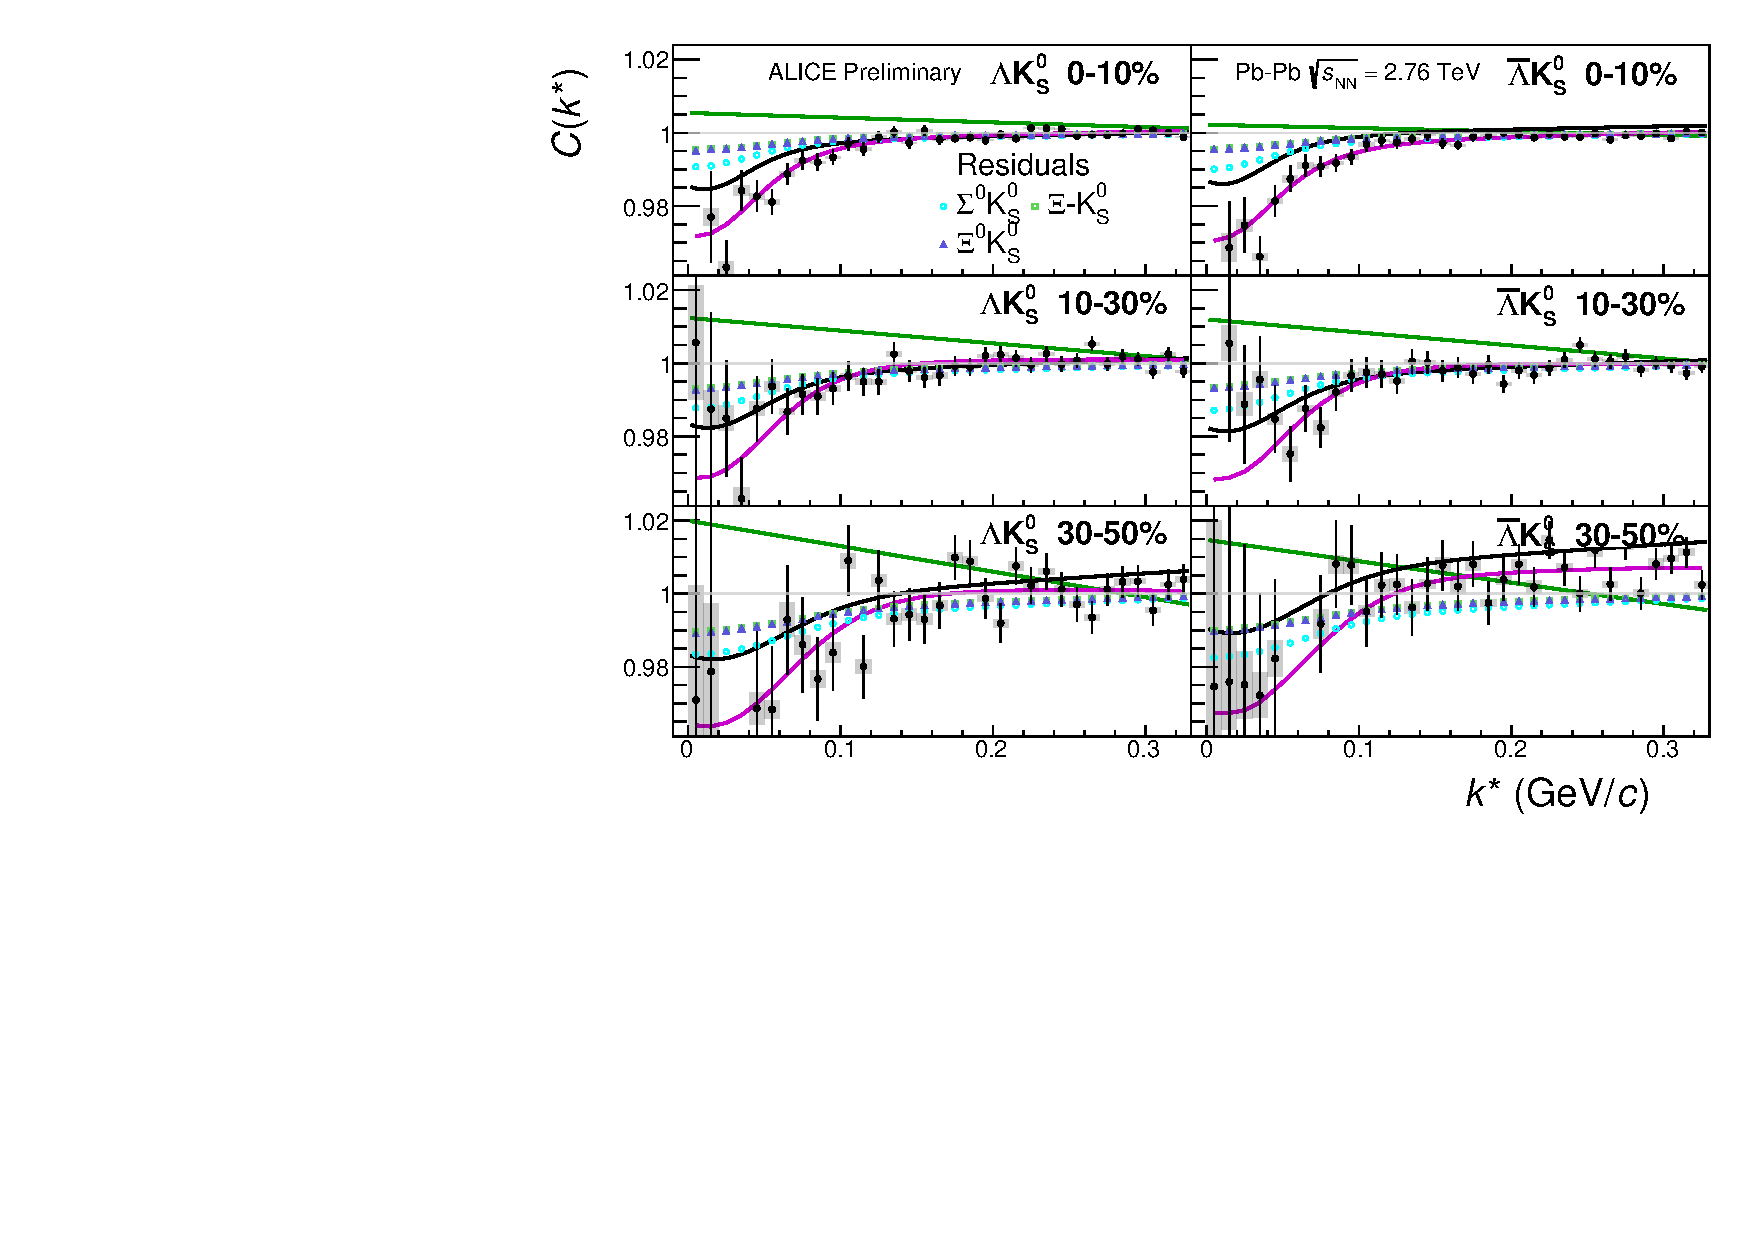
\includegraphics[width=\textwidth]{\ResultsDirLamKs Residuals_3Res/LamK0/canKStarCfwFitsAndResidualsLamK0wConj_0010_1030_3050_ZoomResiduals_MomResCrctn_NonFlatBgdCrctn_SingleLamParam_3Res_PrimMaxDecay4fm_UsingXiDataAndCoulombOnly.pdf}
  \caption[Small Caption]{Caption}
  \label{fig:LamK0wConjFitsAndResiduals_3Res}
\end{figure}



\begin{figure}[h]
  \centering
  \includegraphics[width=\textwidth]{\ResultsDirLamKch canKStarCfwFitsLamKchPwConj_0010_1030_3050_MomResCrctn_NonFlatBgdCrctn_3Res_PrimMaxDecay4fm_UsingXiDataAndCoulombOnly.pdf}
  \caption[\LamKchPALamKchM Fits with 3 Residuals]{Fits, with 3 residual correlations included, to the \LamKchP (left) and \ALamKchM (right) data for the centralities 0-10\% (top), 10-30\% (middle), and 30-50\% (bottom).
The lines represent the statistical errors, while the boxes represent the systematic errors.  
Each has unique $\lambda$ and normalization parameters.
The radii are shared amongst like centralities; the scattering parameters ($\mathbb{R}f_{0}$, $\mathbb{I}f_{0}$, $d_{0}$) are shared amongst all.
The black solid line represents the ``raw" fit, i.e. not corrected for momentum resolution effects nor non-flat background.  
The green line shows the fit to the non-flat background.
The purple points show the fit after momentum resolution and non-flat background corrections have been applied.
The initial values of the parameters is listed, as well as the final fit values with uncertainties.}
  \label{fig:LamKchPwConjFits_3Res}
\end{figure}

\begin{comment}
\begin{figure}[h]
  \centering
  \includegraphics[width=\textwidth]{\ResultsDirLamKch canKStarCfwFitsLamKchPwConj_0010_1030_3050UnZoomed_MomResCrctn_NonFlatBgdCrctn_3Res_PrimMaxDecay4fm_UsingXiDataAndCoulombOnly.pdf}
  \caption[\LamKchPALamKchM Fits with 3 Residuals (Wide Range)]{Same as Fig. \ref{fig:LamKchPwConjFits_3Res}, but with a wider range of view.
Fits, with 3 residual correlations included, to the \LamKchP (left) and \ALamKchM (right) data for the centralities 0-10\% (top), 10-30\% (middle), and 30-50\% (bottom).
The lines represent the statistical errors, while the boxes represent the systematic errors.  
Each has unique $\lambda$ and normalization parameters.
The radii are shared amongst like centralities; the scattering parameters ($\mathbb{R}f_{0}$, $\mathbb{I}f_{0}$, $d_{0}$) are shared amongst all.
The black solid line represents the ``raw" fit, i.e. not corrected for momentum resolution effects nor non-flat background.  
The green line shows the fit to the non-flat background.
The purple points show the fit after momentum resolution and non-flat background corrections have been applied.
The initial values of the parameters is listed, as well as the final fit values with uncertainties.}
  \label{fig:LamKchPwConjFitsUnZoomed_3Res}
\end{figure}
\end{comment}

\begin{figure}[h]
  \centering
  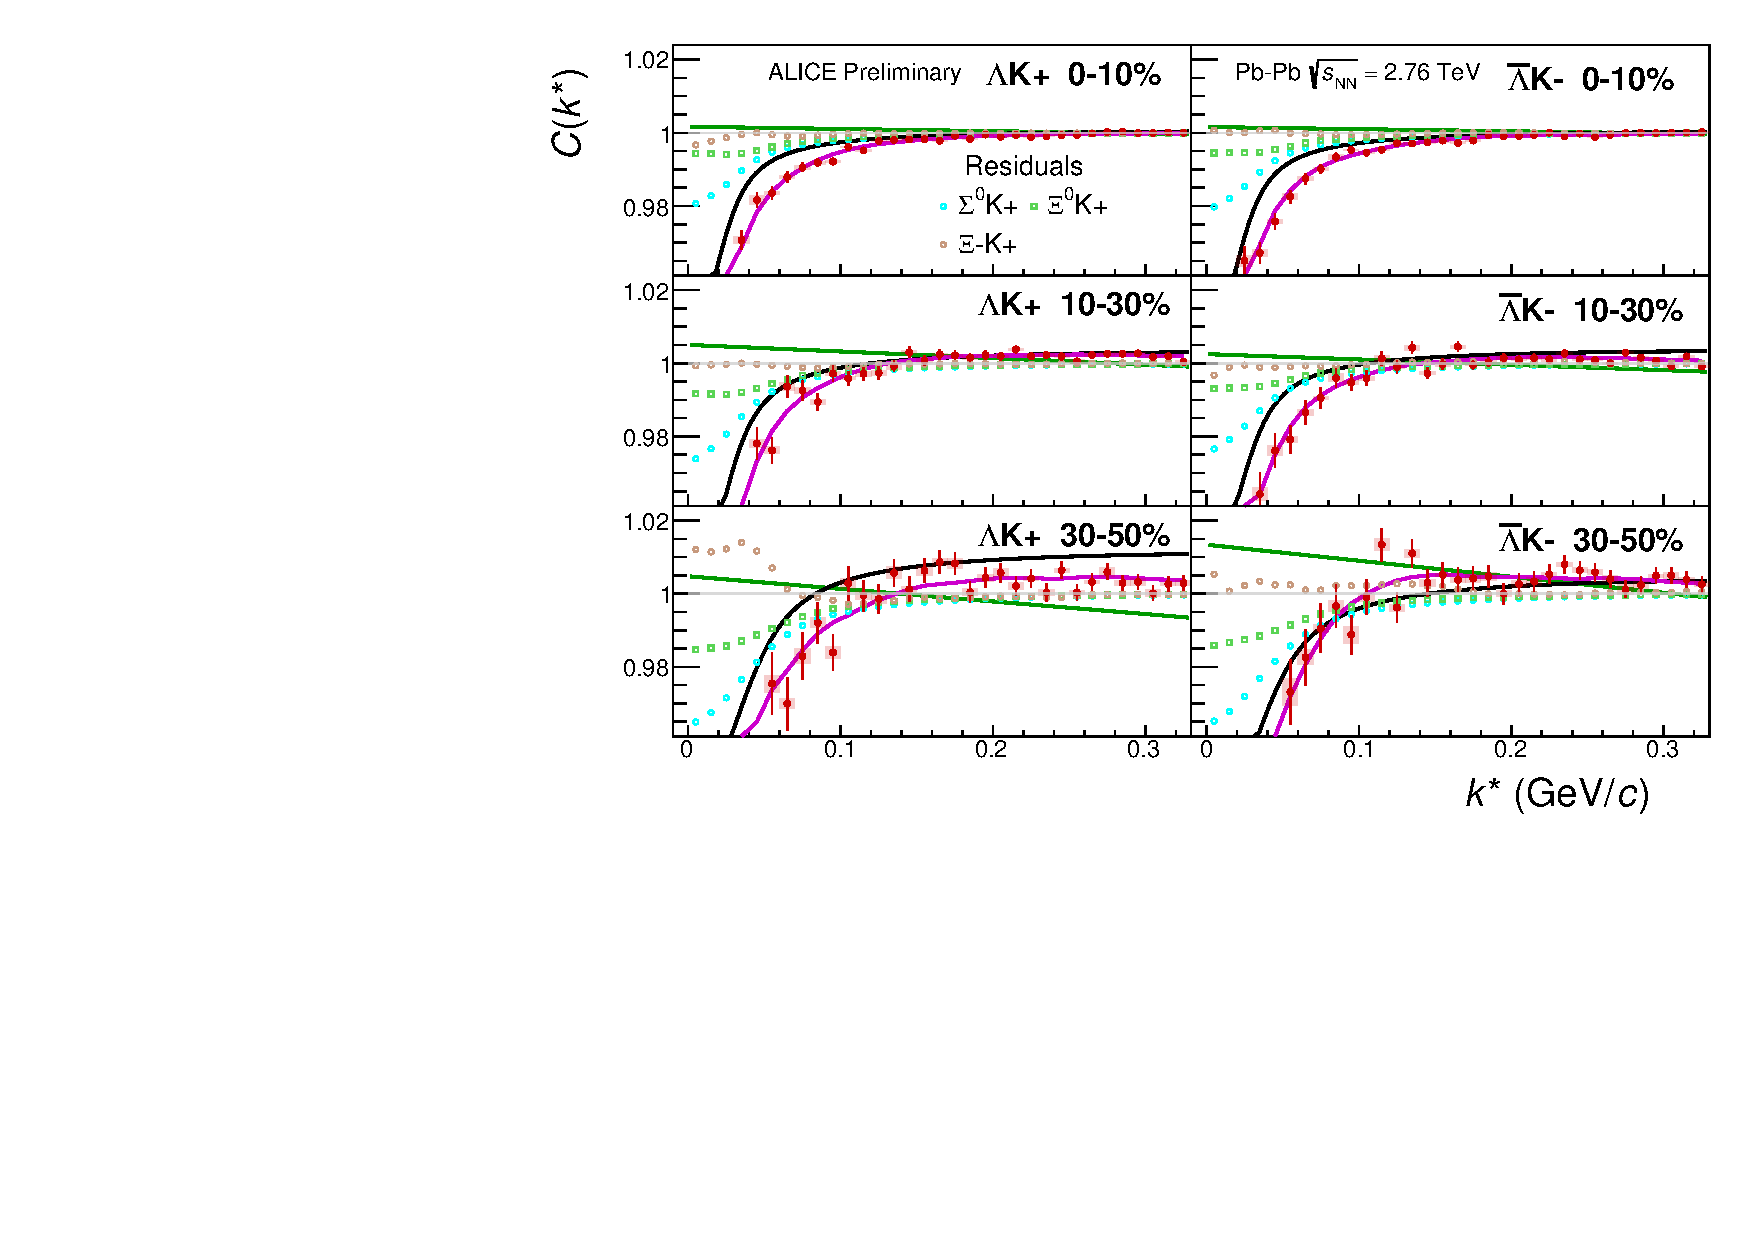
\includegraphics[width=\textwidth]{\ResultsDirLamKch Residuals_3Res/LamKchP/canKStarCfwFitsAndResidualsLamKchPwConj_0010_1030_3050_ZoomResiduals_MomResCrctn_NonFlatBgdCrctn_3Res_PrimMaxDecay4fm_UsingXiDataAndCoulombOnly.pdf}
  \caption[Small Caption]{Caption}
  \label{fig:LamKchPwConjFitsAndResiduals_3Res}
\end{figure}



\begin{figure}[h]
  \centering
  \includegraphics[width=\textwidth]{\ResultsDirLamKch canKStarCfwFitsLamKchMwConj_0010_1030_3050_MomResCrctn_NonFlatBgdCrctn_3Res_PrimMaxDecay4fm_UsingXiDataAndCoulombOnly.pdf}
  \caption[\LamKchMALamKchP Fits with 3 Residuals]{Fits, with 3 residual correlations included, to the \LamKchM(left) with \ALamKchP (right) data for the centralities 0-10\% (top), 10-30\% (middle), and 30-50\% (bottom).
The lines represent the statistical errors, while the boxes represent the systematic errors.  
Each has unique $\lambda$ and normalization parameters.
The radii are shared amongst like centralities; the scattering parameters ($\mathbb{R}f_{0}$, $\mathbb{I}f_{0}$, $d_{0}$) are shared amongst all.
The black solid line represents the ``raw" fit, i.e. not corrected for momentum resolution effects nor non-flat background.  
The green line shows the fit to the non-flat background.
The purple points show the fit after momentum resolution and non-flat background corrections have been applied.
The initial values of the parameters is listed, as well as the final fit values with uncertainties.}
  \label{fig:LamKchMwConjFits_3Res}
\end{figure}


\begin{comment}
\begin{figure}[h]
  \centering
  \includegraphics[width=\textwidth]{\ResultsDirLamKch canKStarCfwFitsLamKchMwConj_0010_1030_3050UnZoomed_MomResCrctn_NonFlatBgdCrctn_3Res_PrimMaxDecay4fm_UsingXiDataAndCoulombOnly.pdf}
  \caption[\LamKchMALamKchP Fits with 3 Residuals (Wide Range)]{Same as Fig. \ref{fig:LamKchMwConjFits_3Res}, but with a wider range of view.
Fits, with 3 residual correlations included, to the \LamKchM(left) with \ALamKchP (right) data for the centralities 0-10\% (top), 10-30\% (middle), and 30-50\% (bottom).
The lines represent the statistical errors, while the boxes represent the systematic errors.  
Each has unique $\lambda$ and normalization parameters.
The radii are shared amongst like centralities; the scattering parameters ($\mathbb{R}f_{0}$, $\mathbb{I}f_{0}$, $d_{0}$) are shared amongst all.
The black solid line represents the ``raw" fit, i.e. not corrected for momentum resolution effects nor non-flat background.  
The green line shows the fit to the non-flat background.
The purple points show the fit after momentum resolution and non-flat background corrections have been applied.
The initial values of the parameters is listed, as well as the final fit values with uncertainties.}
  \label{fig:LamKchMwConjFitsUnZoomed_3Res}
\end{figure}
\end{comment}

\begin{figure}[h]
  \centering
  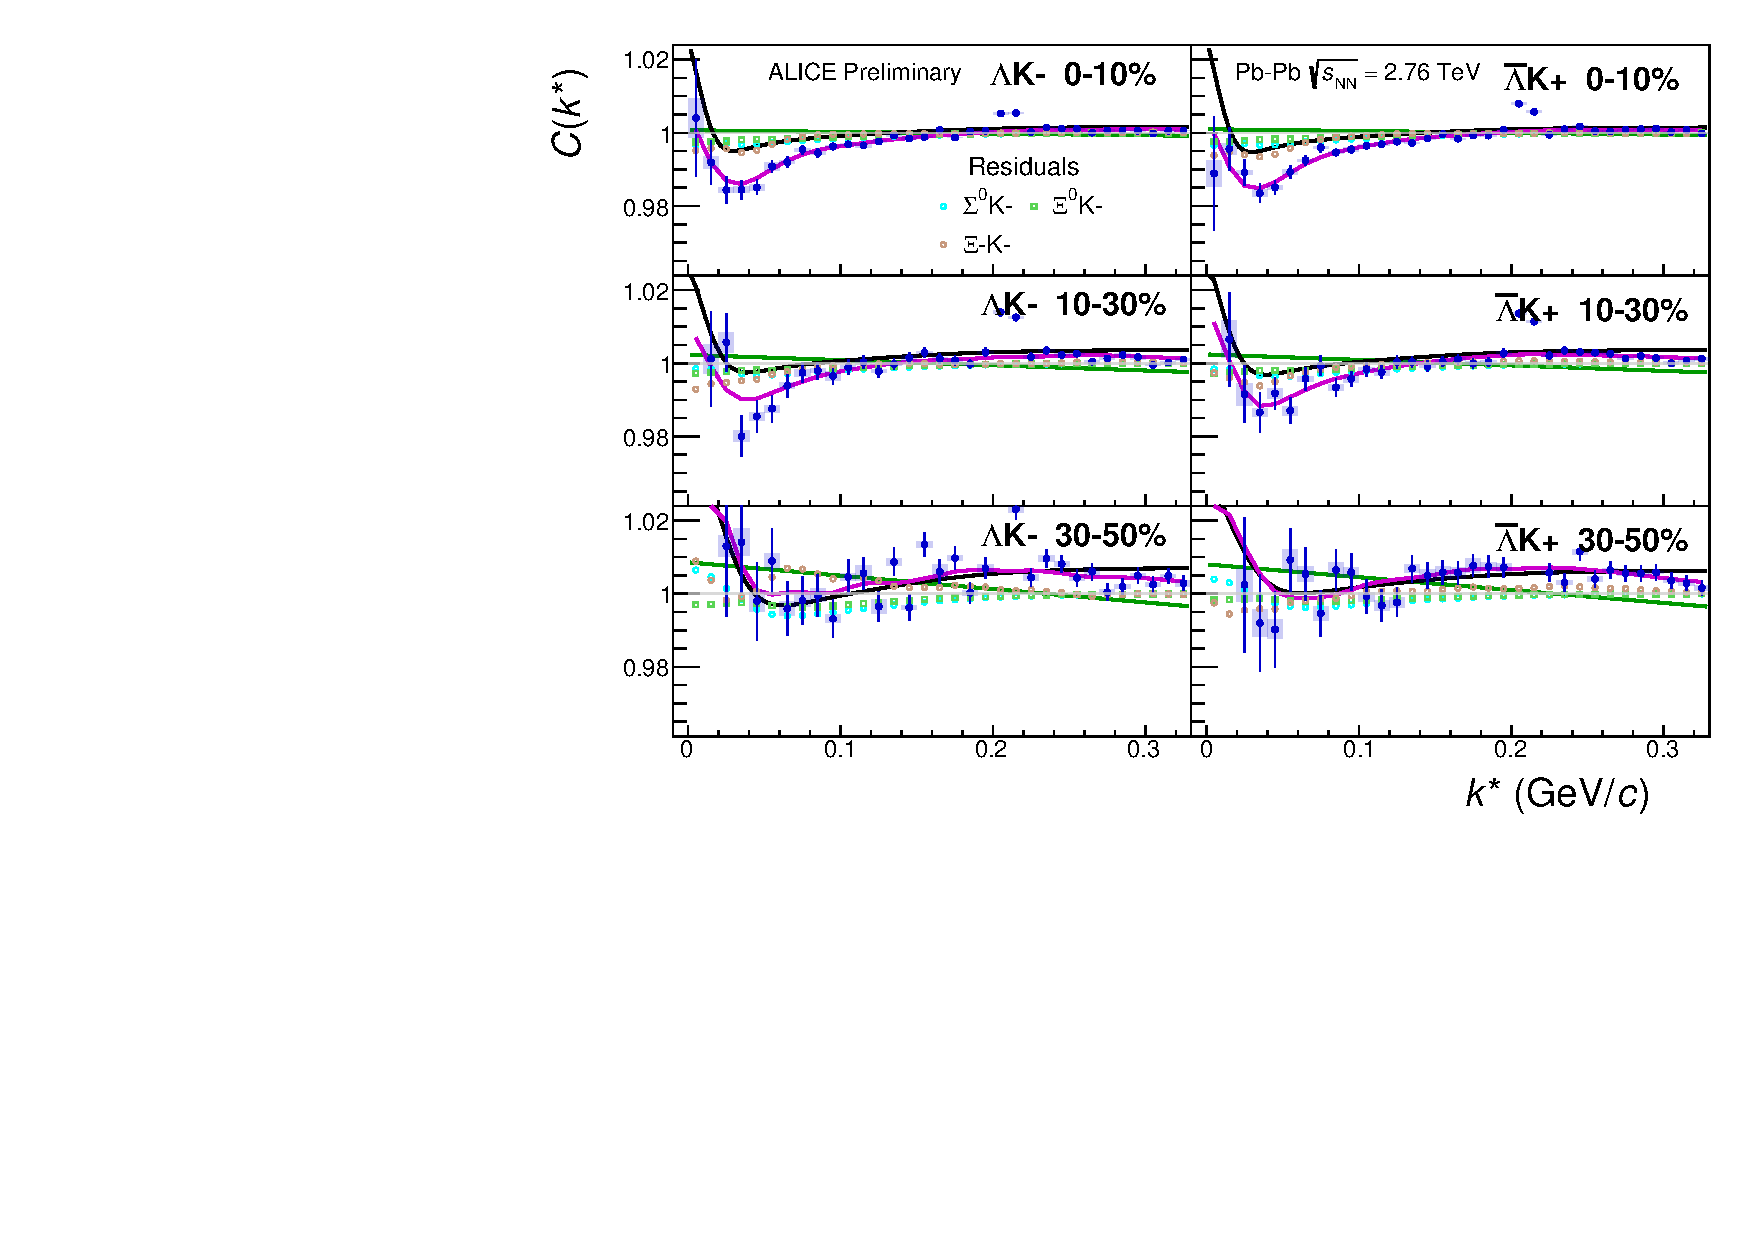
\includegraphics[width=\textwidth]{\ResultsDirLamKch Residuals_3Res/LamKchM/canKStarCfwFitsAndResidualsLamKchMwConj_0010_1030_3050_ZoomResiduals_MomResCrctn_NonFlatBgdCrctn_3Res_PrimMaxDecay4fm_UsingXiDataAndCoulombOnly.pdf}
  \caption[Small Caption]{Caption}
  \label{fig:LamKchMwConjFitsAndResiduals_3Res}
\end{figure}

\pagestyle{empty}
\begin{landscape}

%\clearpage
\begin{table}[htbp]
 \centering
 \resizebox{\paperwidth}{!}{
 \renewcommand{\arraystretch}{1.2}
 \begin{tabular}{|c|c|c|c|c|c|c|}
  \multicolumn{7}{c}{Fit Results \LamALamKs} \\
  \hline
  \multirow{3}{*}{System} & \multirow{3}{*}{Centrality} & \multicolumn{5}{c|}{Fit Parameters} \\
  \cline{3-7}
   & & $\lambda$ & $R$ & $\mathbb{R}f_{0}$ & $\mathbb{I}f_{0}$ & $d_{0}$ \\
  \hline  
  \multirow{3}{*}{\LamKs \& \ALamKs}  
     & 0-10\%
     & \multirow{3}{*}{0.60 $\pm$ 0.63 (stat.) $\pm$ 0.16 (sys.)}    %Lambda (LamK0 & ALamK0 AllCent)
     & 2.78 $\pm$ 0.45 (stat.) $\pm$ 0.33 (sys.)                     %Radius (LamK0 & ALamK0 0010)
     & \multirow{3}{*}{-0.41 $\pm$ 0.10 (stat.) $\pm$ 0.16 (sys.)}   %Ref0   (LamK0 & ALamK0)
     & \multirow{3}{*}{0.20 $\pm$ 0.10 (stat.) $\pm$ 0.13 (sys.)}    %Imf0   (LamK0 & ALamK0)
     & \multirow{3}{*}{2.08 $\pm$ 0.39 (stat.) $\pm$ 0.62 (sys.)} \\ %d0     (LamK0 & ALamK0)
   
     & 10-30\%
     & & 2.22 $\pm$ 0.37 (stat.) $\pm$ 0.23 (sys.)                   %Radius (LamK0 & ALamK0 1030)
     & & & \\
   
     & 30-50\%
     & & 1.68 $\pm$ 0.28 (stat.) $\pm$ 0.11 (sys.)                   %Radius (LamK0 & ALamK0 3050)
     & & & \\
   \hline
 \end{tabular}}
 \caption{Fit Results \LamALamKs, with 3 residual correlations included. 
 Each pair is fit simultaneously with its conjugate (ie. \LamKs with \ALamKs) across all centralities (0-10\%, 10-30\%, 30-50\%), for a total of 6 simultaneous analyses in the fit.
 Each analysis has a unique $\lambda$ and normalization parameter.
 The radii are shared between analyses of like centrality, as these should have similar source sizes.
 The scattering parameters ($\mathbb{R}f_{0}$, $\mathbb{I}f_{0}$, $d_{0}$) are shared amongst all.
 The fit is done on the data with only statistical error bars.
 The errors marked as ``stat." are those returned by MINUIT.
 The errors marked as ``sys." are those which result from my systematic analysis (as outlined in Section \ref{SystematicErrors}).}
 \label{tab:FitResultsLamK0_3Res}
\end{table}  



%\end{landscape}
%\pagestyle{plain}

%\pagestyle{empty}
%\begin{landscape}

\clearpage
\begin{table}[htbp]
 \centering
 \resizebox{\paperwidth}{!}{
 \renewcommand{\arraystretch}{1.2}
 \begin{tabular}{|c|c|c|c|c|c|c|c|}
  \multicolumn{8}{c}{Fit Results \LamALamKpm} \\
  \hline
  \multirow{3}{*}{System} & \multirow{3}{*}{Centrality} & \multirow{3}{*}{Pair Type} & \multicolumn{5}{c|}{Fit Parameters} \\
  \cline{4-8}
   & & & $\lambda$ & $R$ & $\mathbb{R}f_{0}$ & $\mathbb{I}f_{0}$ & $d_{0}$ \\
  \hline  
  \multirow{6}{*}{\LamKchP \& \ALamKchM}  
   & \multirow{2}{*}{0-10\%} 
     & \LamKchP
     & 1.53 $\pm$ 0.56 (stat.) $\pm$ 0.28 (sys.)                     %Lambda (LamKchP 0010)
     & \multirow{2}{*}{5.43 $\pm$ 1.09 (stat.) $\pm$ 0.54 (sys.)}    %Radius (LamKchP & ALamKchM 0010)
     & \multirow{6}{*}{-1.16 $\pm$ 0.25 (stat.) $\pm$ 0.36 (sys.)}   %Ref0   (LamKchP & ALamKchM)
     & \multirow{6}{*}{0.51 $\pm$ 0.28 (stat.) $\pm$ 0.23 (sys.)}    %Imf0   (LamKchP & ALamKchM)
     & \multirow{6}{*}{1.08 $\pm$ 0.43 (stat.) $\pm$ 0.53 (sys.)} \\ %d0     (LamKchP & ALamKchM)
     
     & & \ALamKchM 
     & 1.53 $\pm$ 0.57 (stat.) $\pm$ 0.33 (sys.)                     %Lambda (ALamKchM 0010)
     & & & & \\          
   \cline{2-5}
   
   & \multirow{2}{*}{10-30\%}
     & \LamKchP
     & 1.62 $\pm$ 0.58 (stat.) $\pm$ 0.36 (sys.)                     %Lambda (LamKchP 1030)
     & \multirow{2}{*}{4.75 $\pm$ 0.82 (stat.) $\pm$ 0.42 (sys.)}    %Radius (LamKchP & ALamKchM 1030) 
     & & & \\
             
     & & \ALamKchM 
     & 1.39 $\pm$ 0.49 (stat.) $\pm$ 0.29 (sys.)                     %Lambda (ALamKchM 1030)
     & & & & \\  
   \cline{2-5}
   
   & \multirow{2}{*}{30-50\%}
     & \LamKchP
     & 1.21 $\pm$ 0.31 (stat.) $\pm$ 0.31 (sys.)                     %Lambda (LamKchP 3050)
     & \multirow{2}{*}{3.22 $\pm$ 0.41 (stat.) $\pm$ 0.32 (sys.)}    %Radius (LamKchP & ALamKchM 3050)
     & & & \\
             
     & & \ALamKchM
     & 1.17 $\pm$ 0.30 (stat.) $\pm$ 0.19 (sys.)                     %Lambda (ALamKchM 3050)
     & & & & \\  
   \hline
   \hline
  \multirow{6}{*}{\LamKchM \& \ALamKchP}  
   & \multirow{2}{*}{0-10\%} 
     & \LamKchM
     & 1.91 $\pm$ 0.60 (stat.) $\pm$ 0.24 (sys.)                      %Lambda (LamKchM 0010)
     & \multirow{2}{*}{6.25 $\pm$ 1.08 (stat.) $\pm$ 0.81 (sys.)}     %Radius (LamKchM & ALamKchP 0010)
     & \multirow{6}{*}{0.41 $\pm$ 0.18 (stat.) $\pm$ 0.14 (sys.)}     %Ref0   (LamKchM & ALamKchP)
     & \multirow{6}{*}{0.47 $\pm$ 0.15 (stat.) $\pm$ 0.11 (sys.)}     %Imf0   (LamKchM & ALamKchP)
     & \multirow{6}{*}{-4.89 $\pm$ 2.16 (stat.) $\pm$ 1.33 (sys.)} \\ %d0     (LamKchM & ALamKchP)
     
     & & \ALamKchP 
     & 1.90 $\pm$ 0.57 (stat.) $\pm$ 0.27 (sys.)                      %Lambda (ALamKchP 0010)
     & & & & \\          
   \cline{2-5}
   
   & \multirow{2}{*}{10-30\%}
     & \LamKchM
     & 1.39 $\pm$ 0.43 (stat.) $\pm$ 0.27 (sys.)                      %Lambda (LamKchM 1030) 
     & \multirow{2}{*}{4.74 $\pm$ 0.86 (stat.) $\pm$ 0.60 (sys.)}     %Radius (LamKchM & ALamKchP 1030)
     & & & \\
             
     & & \ALamKchP 
     & 1.50 $\pm$ 0.46 (stat.) $\pm$ 0.26 (sys.)                      %Lambda (ALamKchP 1030)
     & & & & \\  
   \cline{2-5}
   
   & \multirow{2}{*}{30-50\%}
     & \LamKchM
     & 1.57 $\pm$ 0.82 (stat.) $\pm$ 0.57 (sys.)                      %Lambda (LamKchM 3050) 
     & \multirow{2}{*}{2.98 $\pm$ 0.61 (stat.) $\pm$ 0.38 (sys.)}     %Radius (LamKchM & ALamKchP 3050)
     & & & \\
             
     & & \ALamKchP 
     & 0.92 $\pm$ 0.31 (stat.) $\pm$ 0.37 (sys.)                      %Lambda (ALamKchP 3050)
     & & & & \\     
   \hline
 \end{tabular}}
 \caption{Fit Results \LamALamKpm, with 3 residual correlations included.
 Each pair is fit simultaneously with its conjugate (ie. \LamKchP with \ALamKchM and \LamKchM with \ALamKchP) across all centralities (0-10\%, 10-30\%, 30-50\%), for a total of 6 simultaneous analyses in the fit.
 Each analysis has a unique $\lambda$ and normalization parameter.
 The radii are shared between analyses of like centrality, as these should have similar source sizes.
 The scattering parameters ($\mathbb{R}f_{0}$, $\mathbb{I}f_{0}$, $d_{0}$) are shared amongst all.
 The fit is done on the data with only statistical error bars.
 The errors marked as ``stat." are those returned by MINUIT.
 The errors marked as ``sys." are those which result from my systematic analysis (as outlined in Section \ref{SystematicErrors}).}
 \label{tab:FitResultsLamKch_3Res}
\end{table}  

%%%%%%%%%%%%%%%%%%%%%%%%%%%%%%%%%%%%%%%%%%%%%%%%%%%%%%%%%%%%%%%%%%%%%%%%%%%%%%%%%%%%%%%%%%%%%
%%%%%%%%%%%%%%%%%% QM 17 Stuff %%%%%%%%%%%%%%%%%%%%%%%%%%%%%%%%%%%%%%%%%%%%%%%%%%%%%%%%%%%%%%

\clearpage
\begin{table}[htbp]
 \centering
 \resizebox{\paperwidth}{!}{
 \begin{tabular}{|c|c|c|c|c|}
  \multicolumn{2}{c}{} & \multicolumn{3}{c}{\textbf{\large Fit Parameters} (\large \textbf{value $\pm$ statistical error $\pm$ systematic error)}} \\
  \hline
  \textbf{\large Pair Type} & \textbf{\large Centrality} & \multicolumn{3}{c|}{\textbf{\large R}} \\
  \cline{1-5}
  \multirow{5}{*}{\large \textbf{\LamKchP \& \ALamKchM}}
  &  \textbf{0-10\%} & \multicolumn{3}{c|}{\textbf{5.43 $\pm$ 1.09 $\pm$ 0.54}} \\  %Radius
  & \textbf{10-30\%} & \multicolumn{3}{c|}{\textbf{4.75 $\pm$ 0.82 $\pm$ 0.42}} \\  %Radius
  & \textbf{30-50\%} & \multicolumn{3}{c|}{\textbf{3.22 $\pm$ 0.41 $\pm$ 0.32}} \\  %Radius
  \cline{2-5}
  & & \large $\mathbf{\Re f_{0}}$ & \large $\mathbf{\Im f_{0}}$ & \large $\mathbf{d_{0}}$ \\
  \cline{3-5}  
  & & \textbf{-1.16 $\pm$ 0.25 $\pm$ 0.36} & \textbf{0.51 $\pm$ 0.28 $\pm$ 0.23} & \textbf{1.08 $\pm$ 0.43 $\pm$ 0.53} \\
  
  \hline
  \hline
  
  \multirow{5}{*}{\large \textbf{\LamKchM \& \ALamKchP}} 
  &  \textbf{0-10\%} & \multicolumn{3}{c|}{\textbf{6.25 $\pm$ 1.08 $\pm$ 0.81}} \\  %Radius
  & \textbf{10-30\%} & \multicolumn{3}{c|}{\textbf{4.74 $\pm$ 0.86 $\pm$ 0.60}} \\  %Radius
  & \textbf{30-50\%} & \multicolumn{3}{c|}{\textbf{2.98 $\pm$ 0.61 $\pm$ 0.38}} \\  %Radius
  \cline{2-5}
  & & \large $\mathbf{\Re f_{0}}$ & \large $\mathbf{\Im f_{0}}$ & \large $\mathbf{d_{0}}$ \\
  \cline{3-5}     
  & & \textbf{0.41 $\pm$ 0.18 $\pm$ 0.14} & \textbf{0.47 $\pm$ 0.15 $\pm$ 0.11} & \textbf{-4.89 $\pm$ 2.16 $\pm$ 1.33} \\
   
  \hline
  \hline  
  
  \multirow{5}{*}{\large \textbf{\LamKs \& \ALamKs}}  
   &  \textbf{0-10\%} & \multicolumn{3}{c|}{\textbf{2.78 $\pm$ 0.45 $\pm$ 0.33}} \\  %Radius
   & \textbf{10-30\%} & \multicolumn{3}{c|}{\textbf{2.22 $\pm$ 0.37 $\pm$ 0.23}} \\  %Radius
   & \textbf{30-50\%} & \multicolumn{3}{c|}{\textbf{1.68 $\pm$ 0.28 $\pm$ 0.11}} \\  %Radius
   \cline{2-5}   
   & & \large $\mathbf{\Re f_{0}}$ & \large $\mathbf{\Im f_{0}}$ & \large $\mathbf{d_{0}}$ \\
   \cline{3-5} 
   & & \textbf{-0.41 $\pm$ 0.10 $\pm$ 0.16} & \textbf{0.20 $\pm$ 0.10 $\pm$ 0.13} & \textbf{2.08 $\pm$ 0.39 $\pm$ 0.62} \\
  \hline
 \end{tabular}}
 \caption{Fit Results \LamALamKpm and \LamALamKs, with 3 residual correlations included ($\lambda$ parameters not shown).  This table is a condensed version of Tables \ref{tab:FitResultsLamK0_3Res} and \ref{tab:FitResultsLamKch_3Res}} 
 \label{tab:FitResultsLamKCondensed_3Res}
\end{table}

\end{landscape}
\pagestyle{plain}


\begin{figure}[h]
  \centering
  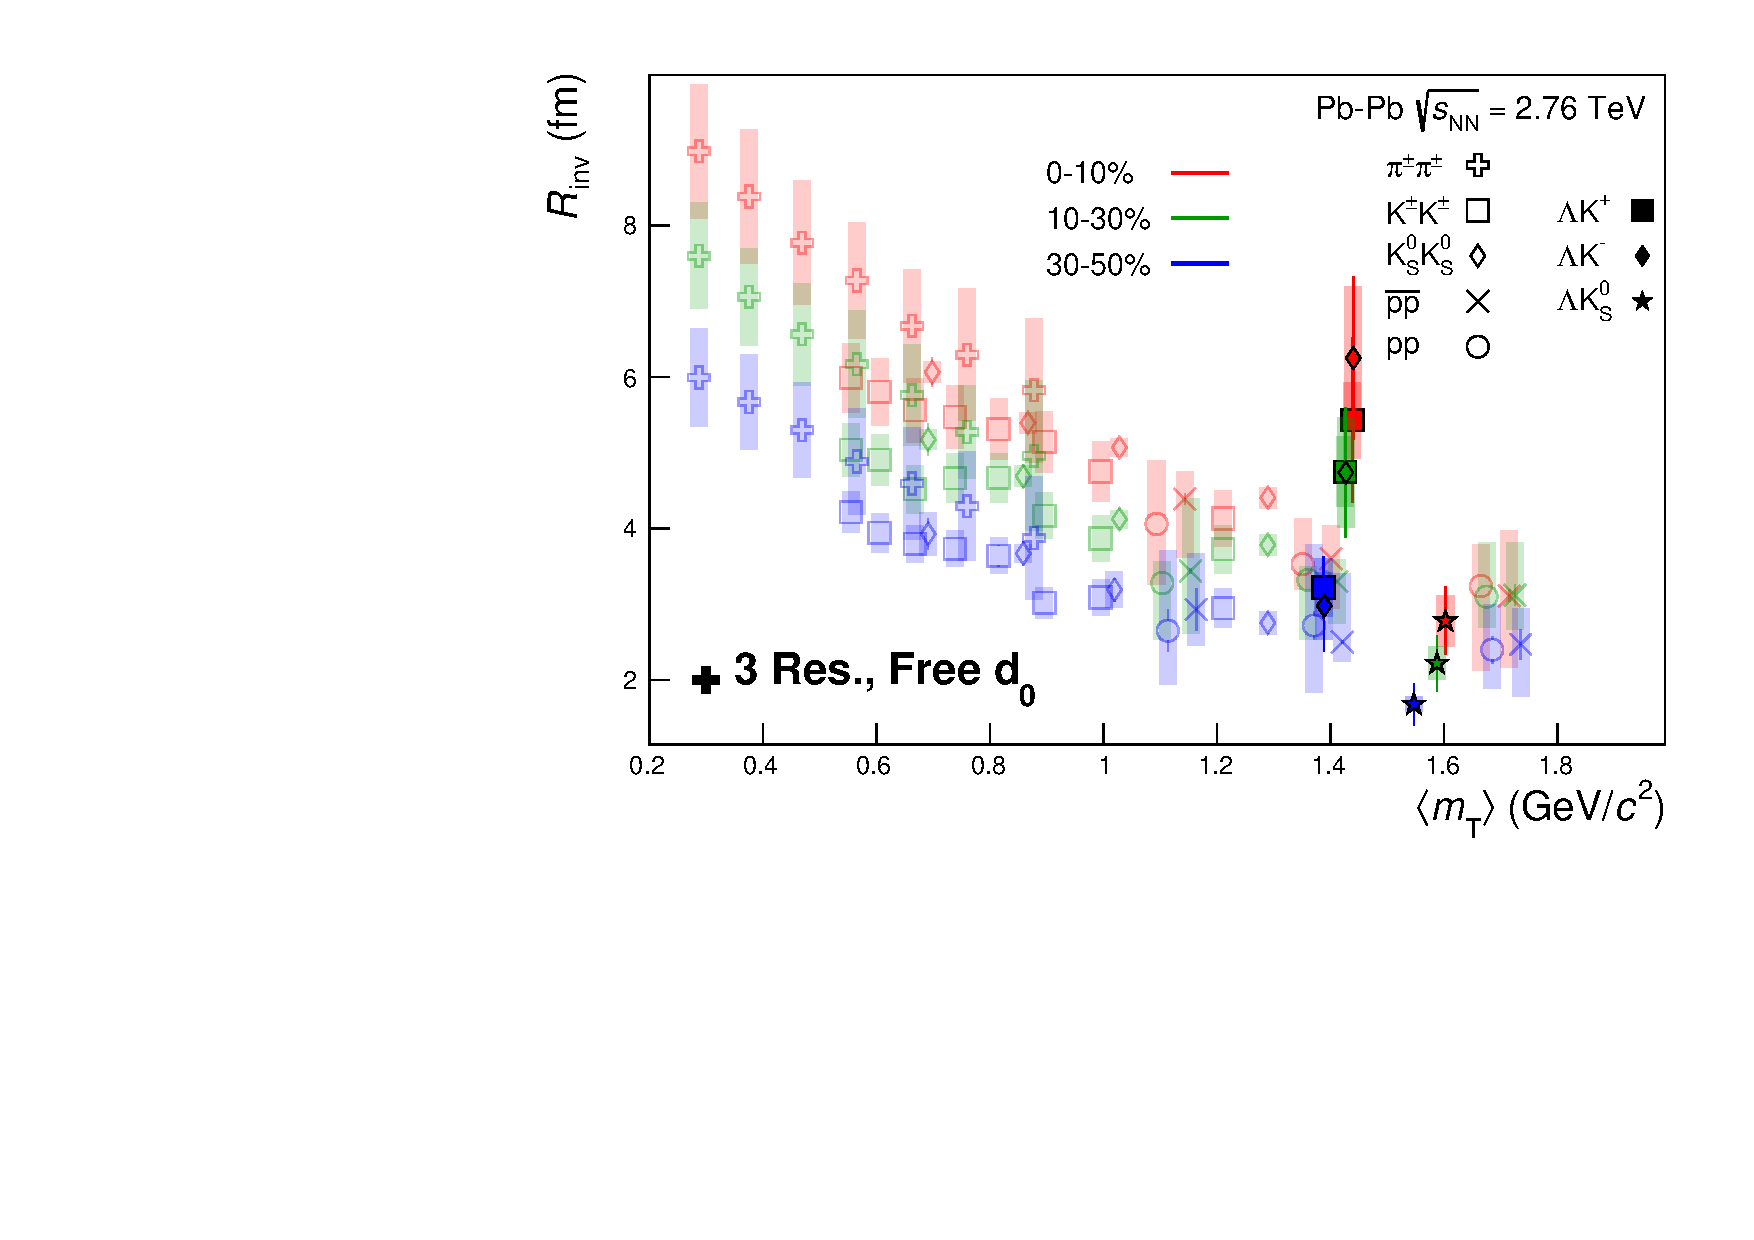
\includegraphics[width=\textwidth]{7_ResultsAndDiscussion/Figures/mTscaling_MinvCalc_OutlinedPoints_OthersTransparent_3Res_FreeD0.pdf}
  \caption[$m_{\mathrm{T}}$ Scaling of Radii: 3 Residuals in Fit]{3 residual correlations in \LamK fits.  Extracted fit $R_{\mathrm{inv}}$ parameters as a function of pair transverse mass ($m_{\mathrm{T}}$) for various pair systems over several centralities. The ALICE published data \cite{Adam:2015vja} is shown with transparent, open symbols.  The new $\Lambda$K results are shown with opaque, filled symbols.  In the left, the \LamKchP (with it's conjugate pair) results are shown separately from the \LamKchM (with it's conjugate pair) results.  In the right, all \LamKpm results are averaged.}
  \label{fig:mTScalingOfRadii_3Res}
\end{figure}

\clearpage


%%%%%%%%%%%%%%%%%%%%%%%%%%%%%%%%%%%%%%%%%%%%%%%%%%%%%%%%%%%%%%%%%%%%%%%%%%%%%%%%%%%%%%%%%%%%%%%%%%%%%%%%%%%%%%%%%%%%%
%%%%%%%%%%%%%%%%%%%%%%%%%%%%%%%%%%%%%%%%%%%% FOR RESULT COMPARISON PURPOSES %%%%%%%%%%%%%%%%%%%%%%%%%%%%%%%%%%%%%%%%%



\clearpage
\begin{table}[htbp]
 \centering
 %------------------------------------LamKchP
% \begin{minipage}{0.3\textwidth}
  \centering
  \renewcommand{\arraystretch}{1.2}
  \begin{tabular}{|c|c|c|c|c|c|}
   \multicolumn{6}{c}{Polynomial Bgds, THERM Bgds fit together} \\
   \hline
   \multirow{3}{*}{\textbf{System}} & \multirow{3}{*}{\textbf{Parameter}} & \multicolumn{4}{c|}{\textbf{Methods}} \\
   \cline{3-6}
    & & Separate & Share R & Share $\lambda_{\mathrm{Conj}}$ & Share Single $\lambda$ \\
   \hline
   \multirow{12}{*}{\LamKchP \& \ALamKchM}
   & $\lambda_{\Lambda\mathrm{K^{+}},0-10\%}$        &  1.70 &  2.18 &  2.16 &  1.92 \\
   & $\lambda_{\bar{\Lambda}\mathrm{K^{-}},0-10\%}$  &  1.72 &  2.21 &  2.16 &  1.92 \\
   \cline{2-6}
   & $\lambda_{\Lambda\mathrm{K^{+}},10-30\%}$       &  1.88 &  1.78 &  1.67 &  1.57 \\
   & $\lambda_{\bar{\Lambda}\mathrm{K^{-}},10-30\%}$ &  1.66 &  1.58 &  1.67 &  1.57 \\
   \cline{2-6}   
   & $\lambda_{\Lambda\mathrm{K^{+}},30-50\%}$       &  1.44 &  1.30 &  1.18 &  1.20 \\
   & $\lambda_{\bar{\Lambda}\mathrm{K^{-}},30-50\%}$ &  1.33 &  1.21 &  1.18 &  1.20 \\  
   \cline{2-6}       
   & $R_{0-10\%}$      &  4.81 &  5.53 &  5.31 &  5.25 \\
   & $R_{10-30\%}$     &  4.38 &  4.37 &  4.22 &  4.26 \\
   & $R_{30-50\%}$     &  3.01 &  2.92 &  2.77 &  2.87 \\
   \cline{2-6}   
   & $\mathbb{R}f_{0}$ & -0.88 & -0.87 & -0.83 & -0.89 \\
   & $\mathbb{I}f_{0}$ &  0.28 &  0.33 &  0.29 &  0.34 \\
   & $d_{0}$           &  1.32 &  1.27 &  1.28 &  1.29 \\
   \hline
   \hline
   \multirow{12}{*}{\LamKchM \& \ALamKchP}
   & $\lambda_{\Lambda\mathrm{K^{-}},0-10\%}$        &  2.20 &  2.10 &  1.91 &  1.92 \\
   & $\lambda_{\bar{\Lambda}\mathrm{K^{+}},0-10\%}$  &  2.19 &  2.10 &  1.91 &  1.92 \\
   \cline{2-6}
   & $\lambda_{\Lambda\mathrm{K^{-}},10-30\%}$       &  1.58 &  1.62 &  1.53 &  1.57 \\
   & $\lambda_{\bar{\Lambda}\mathrm{K^{+}},10-30\%}$ &  1.67 &  1.71 &  1.53 &  1.57 \\
   \cline{2-6}   
   & $\lambda_{\Lambda\mathrm{K^{-}},30-50\%}$       &  1.80 &  2.05 &  1.22 &  1.20 \\
   & $\lambda_{\bar{\Lambda}\mathrm{K^{+}},30-50\%}$ &  1.10 &  1.17 &  1.22 &  1.20 \\  
   \cline{2-6}        
   & $R_{0-10\%}$      &  5.61 &  5.53 &  5.31 &  5.25 \\
   & $R_{10-30\%}$     &  4.20 &  4.37 &  4.22 &  4.26 \\
   & $R_{30-50\%}$     &  2.70 &  2.92 &  2.77 &  2.87 \\
   \cline{2-6}   
   & $\mathbb{R}f_{0}$ &  0.28 &  0.31 &  0.31 &  0.30 \\
   & $\mathbb{I}f_{0}$ &  0.35 &  0.37 &  0.40 &  0.39 \\
   & $d_{0}$           & -5.75 & -5.32 & -4.81 & -4.92 \\
   \hline
  \end{tabular}
% \end{minipage}
 \caption{Comparison: Polynomial non-flat background, THERMINATOR backgrounds fit togethe}
 \label{tab:Comparison_Poly_ThermTogether}
\end{table}



\clearpage
\begin{table}[htbp]
 \centering
 %------------------------------------LamKchP
% \begin{minipage}{0.3\textwidth}
  \centering
  \renewcommand{\arraystretch}{1.5}
  \begin{tabular}{|c|c|c||c|c|c|c|}
   \multicolumn{7}{c}{Polynomial Bgds, THERM Bgds fit together} \\
   \hline
   \multirow{3}{*}{\textbf{Centrality}} & \multirow{3}{*}{\textbf{System}} & \multirow{3}{*}{\textbf{Parameter}} & \multicolumn{4}{c|}{\textbf{Methods}} \\
   \cline{4-7}
    & & & Separate & Share R & Share $\lambda_{\mathrm{Conj}}$ & Share Single $\lambda$ \\ 
   \hline
   
   \multirow{5}{*}{0-10\%} 
   & \LamKchP & $\lambda$  & 1.70 & 2.18 & \multirow{2}{*}{2.16} & \multirow{4}{*}{1.92} \\
   & \ALamKchM & $\lambda$ & 1.72 & 2.21 & & \\
   \cline{2-6}
   & \LamKchM & $\lambda$  & 2.20 & 2.10 & \multirow{2}{*}{1.91} & \\
   & \ALamKchP & $\lambda$ & 2.19 & 2.10 & & \\   
   \cline{2-7}
   & \LamKchP \& \ALamKchM & R & 4.81 & \multirow{2}{*}{5.53} & \multirow{2}{*}{5.31} & \multirow{2}{*}{5.25} \\  
   \cline{2-3} 
   & \LamKchM \& \ALamKchP & R & 5.61 & & & \\  
   \hline
   
   \multirow{5}{*}{10-30\%} 
   & \LamKchP & $\lambda$  & 1.88 & 1.78 & \multirow{2}{*}{1.67} & \multirow{4}{*}{1.57} \\
   & \ALamKchM & $\lambda$ & 1.66 & 1.58 & & \\
   \cline{2-6}
   & \LamKchM & $\lambda$  & 1.58 & 1.62 & \multirow{2}{*}{1.53} & \\
   & \ALamKchP & $\lambda$ & 1.67 & 1.71 & & \\   
   \cline{2-7}
   & \LamKchP \& \ALamKchM & R & 4.38 & \multirow{2}{*}{4.37} & \multirow{2}{*}{4.22} & \multirow{2}{*}{4.26} \\   
   \cline{2-3}
   & \LamKchM \& \ALamKchP & R & 4.20 & & & \\  
   \hline
   
   \multirow{5}{*}{30-50\%} 
   & \LamKchP & $\lambda$  & 1.44 & 1.30 & \multirow{2}{*}{1.18} & \multirow{4}{*}{1.20} \\
   & \ALamKchM & $\lambda$ & 1.33 & 1.21 & & \\
   \cline{2-6}
   & \LamKchM & $\lambda$  & 1.80 & 2.05 & \multirow{2}{*}{1.22} & \\
   & \ALamKchP & $\lambda$ & 1.10 & 1.17 & & \\   
   \cline{2-7}
   & \LamKchP \& \ALamKchM & R & 3.01 & \multirow{2}{*}{2.92} & \multirow{2}{*}{2.77} & \multirow{2}{*}{2.87} \\  
   \cline{2-3} 
   & \LamKchM \& \ALamKchP & R & 2.70 & & & \\  
   \hline
   \hline
   
   & \multirow{3}{*}{\LamKchP \& \ALamKchM} 
   & $\mathbb{R}f_{0}$   & -0.88 & -0.87 & -0.83 & -0.89 \\      
   & & $\mathbb{I}f_{0}$ &  0.28 &  0.33 &  0.29 &  0.34 \\
   & & $d_{0}$           &  1.32 &  1.27 &  1.28 &  1.29 \\
   \hline
   \hline
   
   & \multirow{3}{*}{\LamKchM \& \ALamKchP} 
   & $\mathbb{R}f_{0}$   &  0.28 &  0.31 &  0.31 &  0.30 \\      
   & & $\mathbb{I}f_{0}$ &  0.35 &  0.37 &  0.40 &  0.39 \\
   & & $d_{0}$           & -5.75 & -5.32 & -4.81 & -4.92 \\
   \hline   
  \end{tabular}
% \end{minipage}
 \caption{Comparison: Polynomial non-flat background, THERMINATOR backgrounds fit together}
 \label{tab:Comparison_Poly_ThermTogetherv2}
\end{table}


\end{document}